% !TeX root = ../main.tex
% Add the above to each chapter to make compiling the PDF easier in some editors.

\chapter{Experiments}\label{chapter:introduction}
We evaluate both the 2D and 3D results for our framework, since our model estimate 2D heatmaps and 3D poses. The training set contains sequences: \textit{"170407\_haggling\_a1", "160226\_haggling1", "161202\_haggling1"} and we randomly sample 5 different camera views out of 26 camera views. We choose \textit{"160906\_pizza1"} as the validation sequence and 5 fixed views, \textit{(0, 12), (0, 6), (0, 23), (0, 13), (0, 3)}, that do not exist in the training set.

To compare our framework, we train a baseline model, that has the same structure as the 2d backbone but is train on CMU dataset. Since the CMU dataset has only 3D skeletons, the project groundtruth 2D pose have all the joints annotated. Thus, the baseline model is trained with both occluded and unoccluded joints. Our intuition is the baseline should be able to learn to "see" through the occlusion.

We use Adam optimizer with a learning rate of 0.01 and train every modules, e.g. Baseline Model, 2D backbone, view Fusion, and temporal fusion module, for 20 epochs. During the training, we use the batch size of 32 for all the above mentioned modules except temporal modules due to memory limitation. For temporal module, we use a batch size of 1, where each sample is the tensor with dimension (55, 128, 128, 1, 9), meaning number of keypoints, height, width, number of view, and number of frames.
\section{Quantitative Results}
In 2D evaluation, we use ground truth bounding boxes to localize people in the view. Each bounding box are generated by taking the most top-right and bottom left corners of the 2D pose, projected from the ground-truth 3D pose. After localizing individual with the ground-truth bounding boxes, we take the maximum score within the bounding box for each channel of the heatmap as the joint location and calculate PCKh accordingly.
In 3D evaluation, we assign ground truth 3D poses to the estimated 3D poses using Hungarian algorithm, where the cost is the mean distance of joints difference between the 3D poses of ground truth and predictions. 

\begin{table}
	\centering
	\resizebox{\columnwidth}{!}{%
	\begin{tabular}{l|l|l|l|l|l|l|l|l|l}\toprule
		\textbf{Model} &\textbf{nose} & \textbf{eye\_l} & \textbf{eye\_r} & \textbf{ear\_l} &\textbf{ear\_r}& \textbf{sho\_l}&\textbf{sho\_r}&\textbf{elb\_l}&\textbf{elb\_r}\\\midrule
		Baseline&0.29&0.08&0.23&0.09&0.17&0.22&0.23&0.10&0.15\\\midrule\midrule
		ResNet&0.29&0.08&0.23&0.09&0.17&0.22&0.23&0.10&0.15\\ \hline
		+ View Fusion&     \textbf{0.34}&\textbf{0.35}&\textbf{0.39}&\textbf{0.37}&\textbf{0.40}&0.22&\textbf{0.31}&\textbf{0.13}&\textbf{0.19}\\ \hline
		+ Temporal Fusion&0.27&0.35&0.36&0.35&0.31&0.20&0.29&0.10&0.18\\ \midrule
		\textbf{Model} &\textbf{wri\_l}&\textbf{wri\_r}&\textbf{hip\_l} & \textbf{hip\_r} & \textbf{kne\_l} & \textbf{kne\_r}&\textbf{ank\_l}&\textbf{ank\_r}\\\midrule
		Baseline&0.12&0.16&0.17&0.15&0.13&0.10&0.17&0.13\\\midrule\midrule
		ResNet&            0.12&\textbf{0.16}&0.17&0.15&0.13&0.10&\textbf{0.16}&0.13\\ \hline
		+ View Fusion&     \textbf{0.13}&0.15&\textbf{0.24}&\textbf{0.25}&\textbf{0.17}&\textbf{0.18}&0.13&0.13\\ \hline
		+ Temporal Fusion& 0.11 &0.09&0.20&0.19&0.12&0.13&0.13&0.12\\ \bottomrule
	\end{tabular}
	}
	\caption{2D evaluation based on PCKh@0.5 with 5 views input.}\label{tbl:2d-evaluation-pckh}
\end{table} 

\begin{table}
	\centering
	\resizebox{\columnwidth}{!}{%
		\begin{tabular}{l|l|l|l|l|l|l|l|l|l}\toprule
			\textbf{Model} &\textbf{sho\_l} & \textbf{sho\_r} & \textbf{elb\_l} & \textbf{elb\_r} &\textbf{wri\_l}& \textbf{wri\_r}&\textbf{hip\_l}&\textbf{hip\_r}&\textbf{kne\_l}\\\midrule
			Baseline&0.08&0.17&0.02&0.03&0.01&0.03&0.09&0.09&\textbf{0.02}\\\midrule\midrule
			ResNet&0.07&0.18&0.03&0.06&0.02&0.03&0.09&0.08&0.01\\ \hline
			+ View Fusion&     \textbf{0.15}&\textbf{0.18}&\textbf{0.04}&\textbf{0.09}&\textbf{0.02}&0.03&\textbf{0.13}&\textbf{0.11}&0.01\\ \hline
			+ Temporal Fusion&0.01&0.03&0&0.03&0&0&0.01&0&0\\ \midrule
			\textbf{Model} &\textbf{kne\_r}&\textbf{ank\_l}&\textbf{ank\_r} \\\midrule
			Baseline&0.007&0.006&\textbf{0.006}\\\midrule\midrule
			ResNet&            0.008&0.003&0.004\\ \hline
			+ View Fusion&     \textbf{0.01}&\textbf{0.009}&0.004\\ \hline
			+ Temporal Fusion& 0 &0&0\\ \bottomrule
		\end{tabular}
	}
	\caption{3D evaluation based on PCKh@0.5 and with 5 views input.}\label{tbl:3d-evaluation-pckh}
\end{table} 

\begin{table}
	\centering
	\resizebox{\columnwidth}{!}{%
		\begin{tabular}{lrrrrrrrrrrrrrrrrrr}\toprule
			&\multicolumn{3}{c}{\textbf{sho\_l}}&\multicolumn{3}{c}{\textbf{sho\_r}}&\multicolumn{3}{c}{\textbf{elb\_l}}&\multicolumn{3}{c}{\textbf{elb\_r}}
			\\\cmidrule(r){2-4}\cmidrule(r){5-7}\cmidrule(r){8-10}\cmidrule(r){11-13}     
			& 3 & 4 & 5 & 3 & 4 & 5 & 3 & 4 & 5 & 3 & 4 & 5\\\midrule
			ResNet    & 0.02 & 0.04 & 0.07 &0.03 & 0.1 & \textbf{0.18} & 0.006 & 0.01 & 0.03 &0.007 & 0.03 & 0.06\\ \hline
			+ View Fusion& 0.02 & 0.06 & \textbf{0.15} &0.04 & 0.1 & \textbf{0.18} & 0.006 & 0.02 & \textbf{0.04} &0.01 & 0.04 & \textbf{0.09}\\ \hline
			+ Temporal Fusion& 0.02 & 0.02 & 0.01 &0.05 & 0.09 & 0.03 & 0 & 0 & 0 &0.02 & 0.04 & 0.03\\\midrule
			&\multicolumn{3}{c}{\textbf{wri\_l}}&\multicolumn{3}{c}{\textbf{wri\_r}}&\multicolumn{3}{c}{\textbf{hip\_l}}&\multicolumn{3}{c}{\textbf{hip\_r}}
			\\\cmidrule(r){2-4}\cmidrule(r){5-7}\cmidrule(r){8-10}\cmidrule(r){11-13}     
			& 3 & 4 & 5 & 3 & 4 & 5 & 3 & 4 & 5 & 3 & 4 & 5\\\midrule
			ResNet    & 0.003 & 0.01 & \textbf{0.02} &0.005 & 0.02 & \textbf{0.03} & 0.02 & 0.05 & 0.09 &0.01 & 0.04 & 0.08\\ \hline
			+ View Fusion& 0.004 & 0.02 & \textbf{0.02} &0.004 & 0.02 & \textbf{0.03} & 0.02 & 0.06 & \textbf{0.13} &0.02 & 0.06 & \textbf{0.11}\\ \hline
			+ Temporal Fusion& 0.003 & 0.01 & 0 &0.005 & 0.008 & 0 & 0.005 & 0.01 & 0.01 &0.01 & 0.01 & 0\\ \midrule
			&\multicolumn{3}{c}{\textbf{kne\_l}}&\multicolumn{3}{c}{\textbf{kne\_r}}&\multicolumn{3}{c}{\textbf{ank\_l}}&\multicolumn{3}{c}{\textbf{ank\_r}}
			\\\cmidrule(r){2-4}\cmidrule(r){5-7}\cmidrule(r){8-10}\cmidrule(r){11-13}     
			& 3 & 4 & 5 & 3 & 4 & 5 & 3 & 4 & 5 & 3 & 4 & 5\\\midrule
			ResNet    & 0.001 & 0.007 & \textbf{0.01} &0.003 & 0.004 & 0.008 & 0.0003 & 0.0001 & \textbf{0.003} &0.0006 & 0.0002 & \textbf{0.004}\\ \hline
			+ View Fusion& 0.0003 & 0.008 & \textbf{0.01} &0.0003 & 0.007 & \textbf{0.01} & 0 & 0.0003 & 0.0009 &0.0003 & 0.001 & \textbf{0.004}\\ \hline
			+ Temporal Fusion& 0 & 0.002 & 0 &0 & 0 & 0 & 0 & 0 & 0 &0 & 0 & 0\\ \bottomrule
		\end{tabular}
	}
		\caption{3D evaluation based on PCKh@0.5 with 3, 4 and 5 views input.}\label{tbl:3d-evaluation-views-change}
\end{table} 
\newpage

\section{Qualitative Results}
We show the 2D and 3D prediction of human poses in Fig. \ref{fig:ch6-2d-evaluation} and Fig. \ref{fig:ch6-3d-evaluation}. Note that in 2D, the ground truth bounding boxes are used to localize people in each view.
\begin{figure}
	\centering
	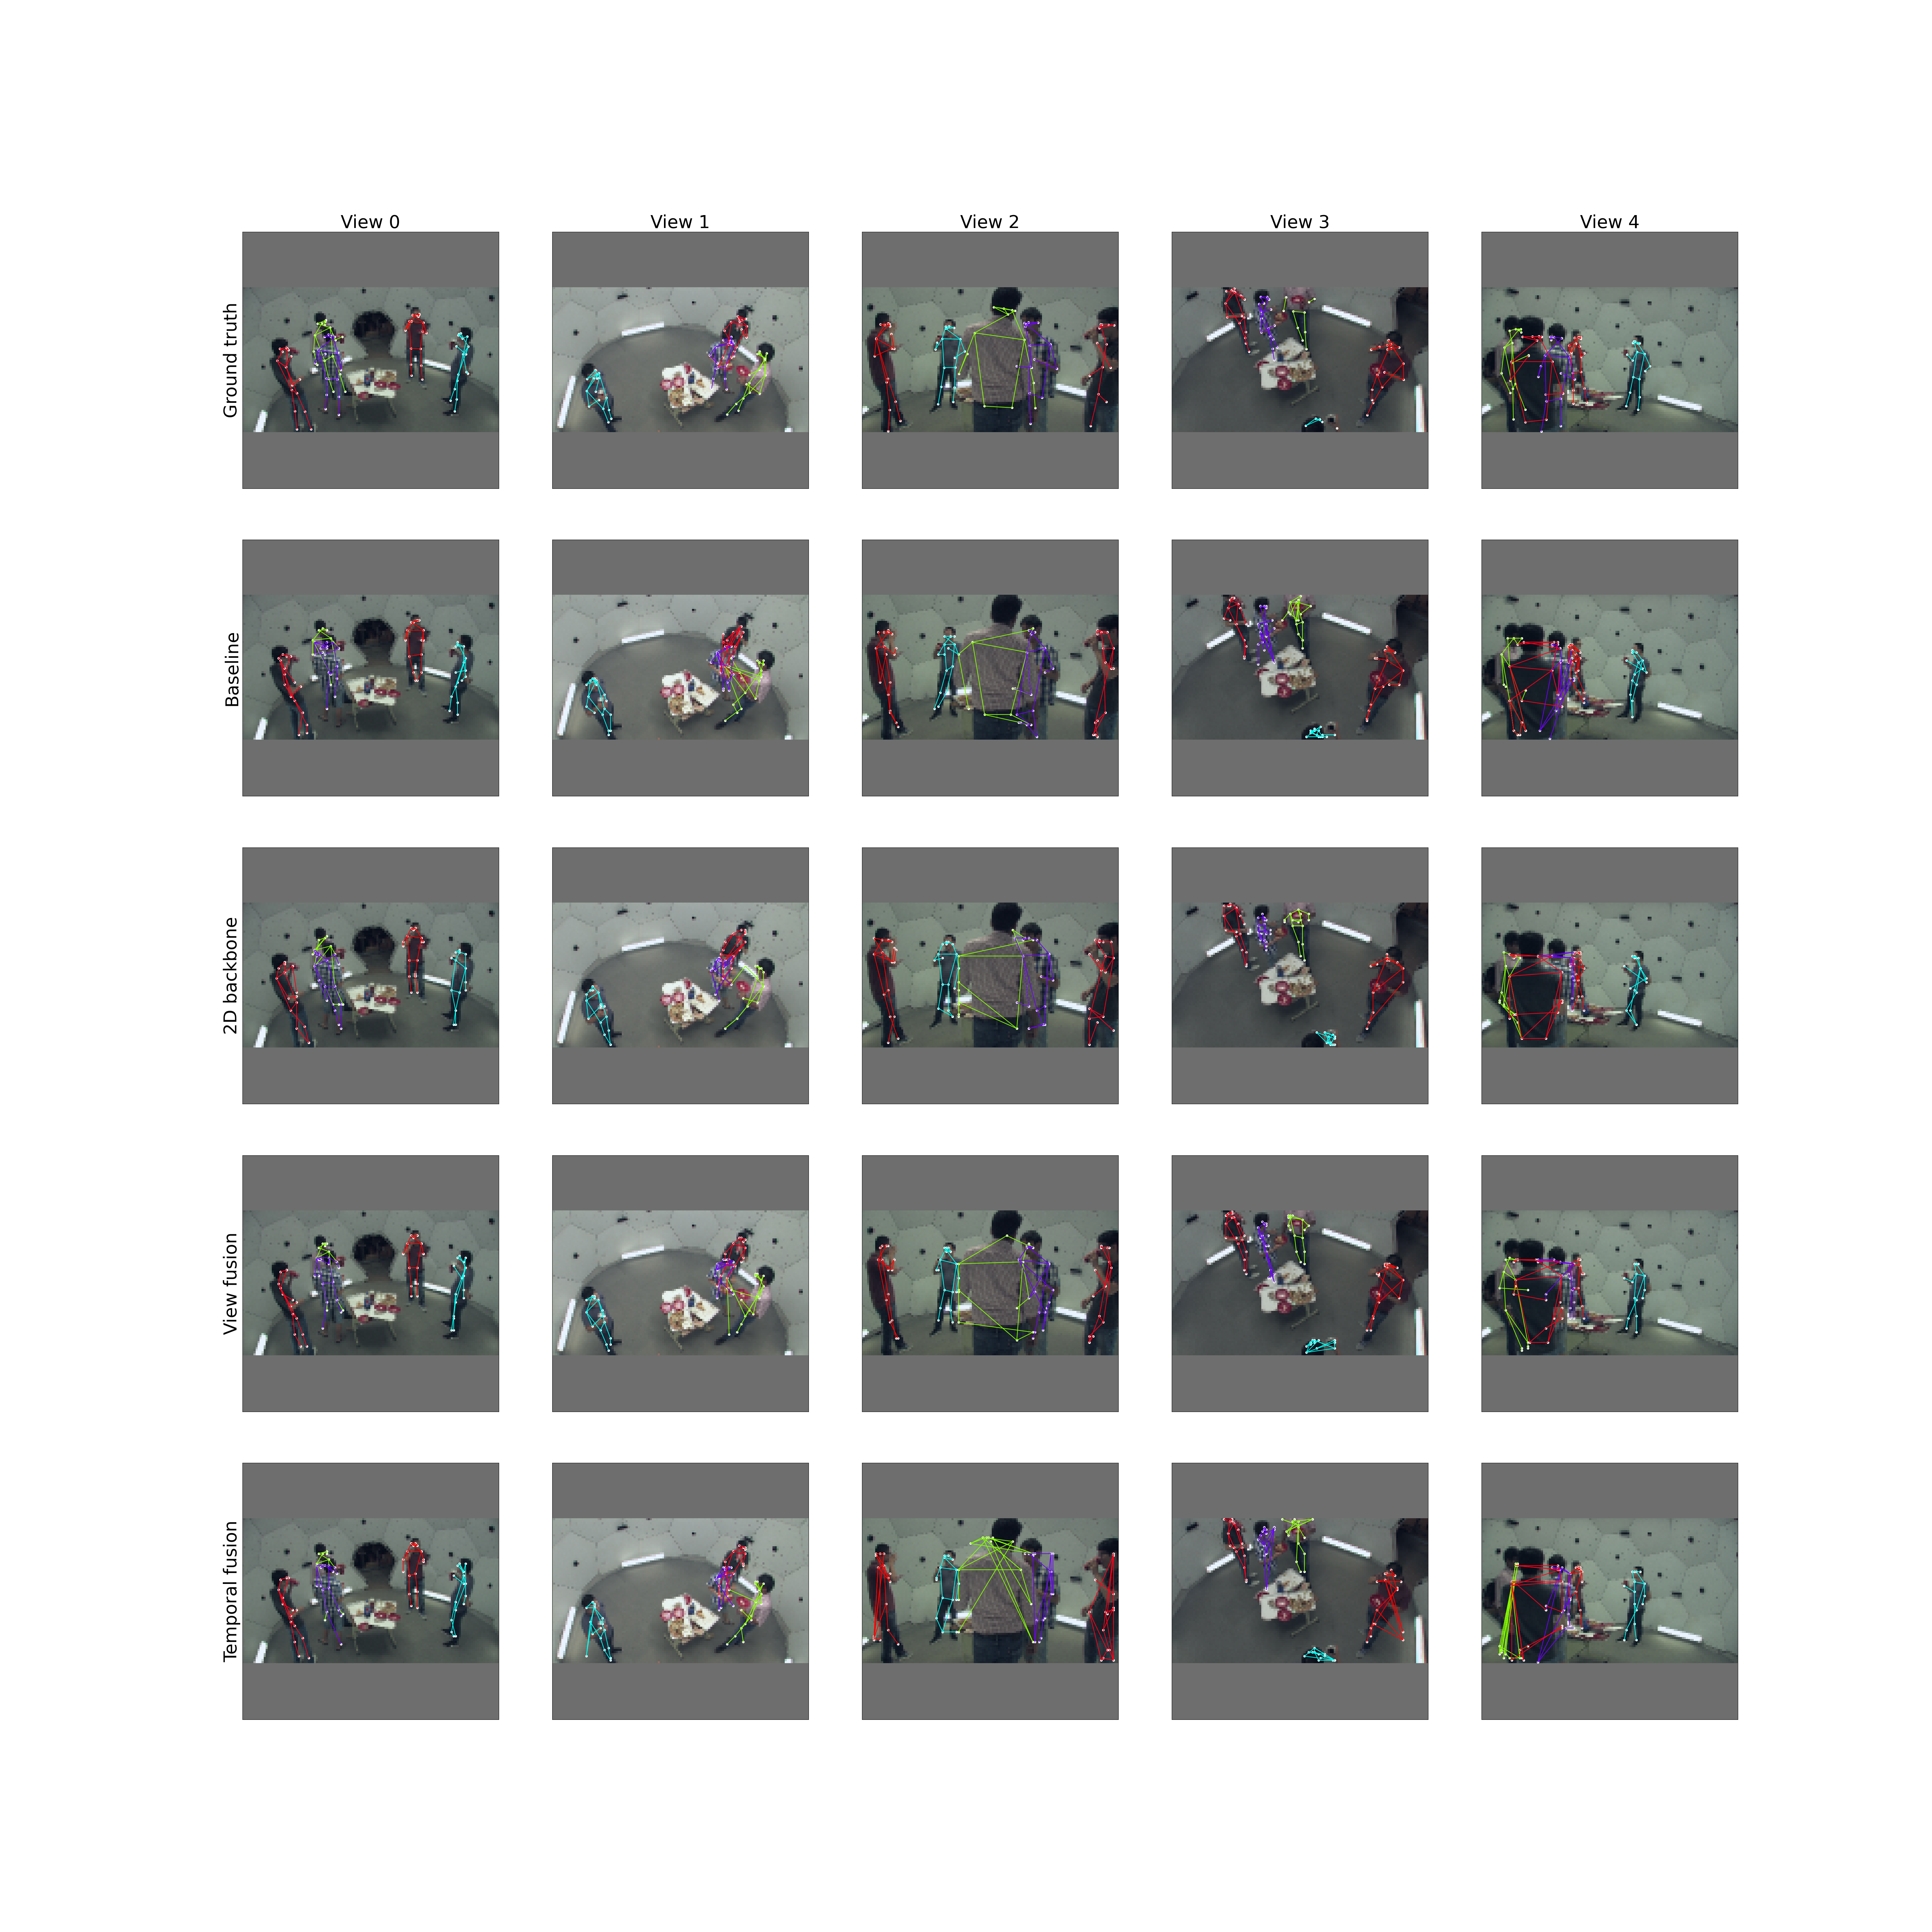
\includegraphics[width=1.0\columnwidth]{figures/ch6/2d-evaluation.png}
	\caption{2d pose estimation results. Better view with PDF and zoom.} 
	\label{fig:ch6-2d-evaluation}
\end{figure}

\begin{figure}
\centering
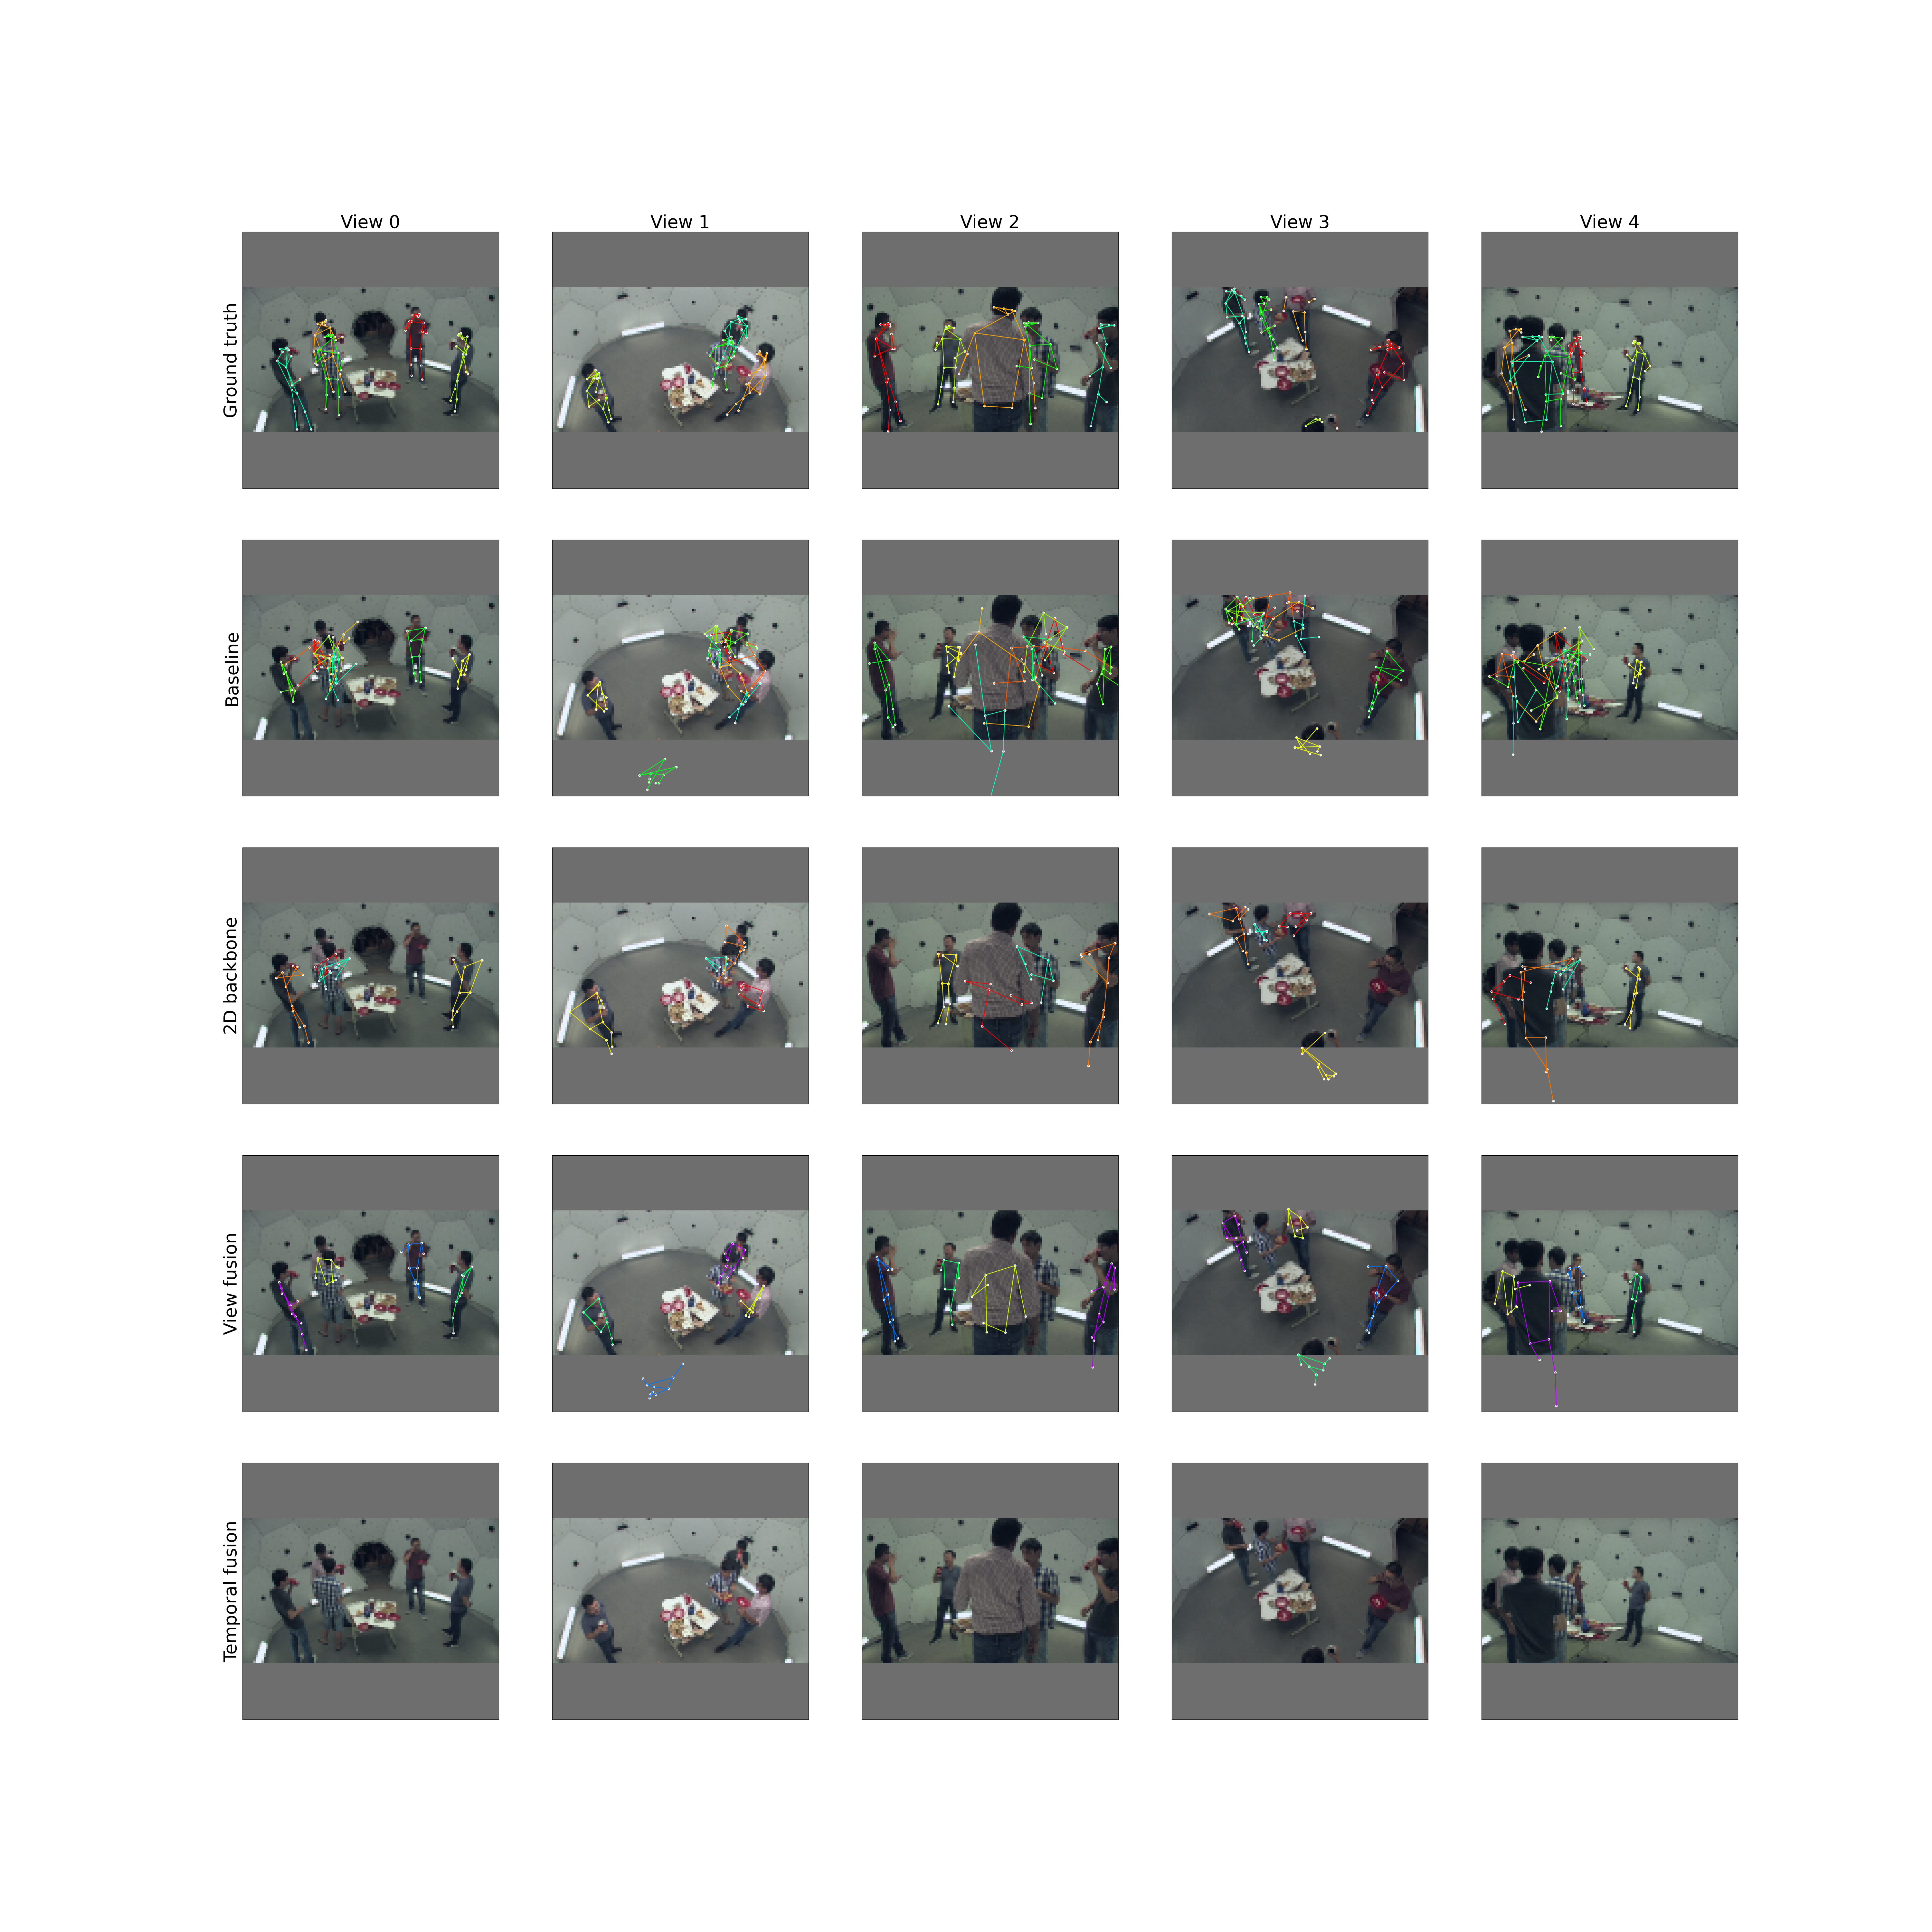
\includegraphics[width=1.0\columnwidth]{figures/ch6/3d-evaluation.png}
\caption{3d pose estimation results. Better view with PDF and zoom.} 
\label{fig:ch6-3d-evaluation}
\end{figure}

\section{Discussion}
We first compare the baseline model with our 2D backbone. Observing on the results shown in Table \ref{tbl:2d-evaluation-pckh} and \ref{tbl:3d-evaluation-pckh}, although baseline and 2D backbone each train on different datasets (one in indoor studio environment with all joints annotated and the other on natural image with some joints missing), both models have very similar performance. This means our 2D backbone generalize well on different dataset and the baseline model does not able to learn seeing through the occlusion.

We observe improvement at almost every type of joint when we combine 2d backbone with view fusion modules in 2D and 3D pose estimation. Especially, combining 2d backbone and view fusion modules help our 3D pose estimation algorithm produce less but more accurate poses, shown in Fig. \ref{fig:ch6-3d-evaluation}. In addition, we also conduct experiments regarding the effect of number of input view to the performance of 3D pose estimation, shown in Table \ref{tbl:3d-evaluation-views-change}. The results support our intuition that the performance of our complete framework can benefit from more views. 

However, we observe that a degradation at the performance of 3d pose estimation when we add temporal fusion module. According to our observation, the temporal module smooth out the peak in the heatmap quite a lot, making the score margin between background and heatmap much smaller. Since our 3D pose estimation algorithm does binary threshold to find peaks first and, then, does triangulation based on the location, the algorithm suffers from a low number of peak. Furthermore, we consider out estimated 3D pose with less than 5 limbs as invalid, so lots of pose are discard, leaving 0 PCKh in detection of some type of joints.